\documentclass[12pt]{article}
\usepackage[utf8]{inputenc}
\usepackage{geometry}
\geometry{letterpaper, margin=0.25in}
\usepackage{graphicx} 
\usepackage{parskip}
\usepackage{booktabs}
\usepackage{array} 
\usepackage{paralist} 
\usepackage{verbatim}
\usepackage{subfig}
\usepackage{fancyhdr}
\usepackage{sectsty}
\usepackage[shortlabels]{enumitem}

\pagestyle{fancy}
\renewcommand{\headrulewidth}{0pt} 
\lhead{}\chead{}\rhead{}
\lfoot{}\cfoot{\thepage}\rfoot{}

%%% ToC (table of contents) APPEARANCE
\usepackage[nottoc,notlof,notlot]{tocbibind} 
\usepackage[titles,subfigure]{tocloft}
\renewcommand{\cftsecfont}{\rmfamily\mdseries\upshape}
\renewcommand{\cftsecpagefont}{\rmfamily\mdseries\upshape} %

\usepackage{amsmath}
\usepackage{amssymb}
\usepackage{mathtools}
\usepackage{empheq}
\usepackage{xcolor}
\usepackage{bbm}
\usepackage{tikz}
\usepackage{pgfplots}
\usepackage{tikz-cd}
\pgfplotsset{compat=1.18}
\usetikzlibrary{intersections, decorations.markings}
\tikzset{
    marking along/.style n args={2}{
        decoration={
                markings, 
                mark=at position #1 with {\arrow{#2}}
        },
        postaction={decorate}
        },
    marking along/.default={0.5}{>}
    wavy/.style={
        decorate,decoration={coil,aspect=0}
    },
    two marks/.style n args={1}{
        decoration={
            markings,
            mark=at position 0.25 with {\arrow{#1}},
            mark=at position 0.75 with {\arrow{#1}}
        },
         postaction={decorate}
    },
    two marks/.default={>}
}

\colorlet{mygreen}{green!50!teal}

\newcommand{\ans}[1]{\boxed{\text{#1}}}
\newcommand{\vecs}[1]{\langle #1\rangle}
\renewcommand{\hat}[1]{\widehat{#1}}

\renewcommand{\P}{\mathbb{P}}
\newcommand{\R}{\mathbb{R}}
\newcommand{\E}{\mathbb{E}}
\newcommand{\Z}{\mathbb{Z}}
\newcommand{\N}{\mathbb{N}}
\newcommand{\Q}{\mathbb{Q}}
\newcommand{\C}{\mathbb{C}}

\newcommand{\ind}{\mathbbm{1}}
\newcommand{\qed}{\quad \blacksquare}

\newcommand{\brak}[1]{\left\langle #1 \right\rangle}
\newcommand{\bra}[1]{\left\langle #1 \right\vert}
\newcommand{\ket}[1]{\left\vert #1 \right\rangle}

\newcommand{\abs}[1]{\left\vert #1 \right\vert}
\newcommand{\mfX}{\mathfrak{X}}
\newcommand{\ep}{\varepsilon}

\newcommand{\Ec}{\mathcal{E}}
\newcommand{\Nc}{\mathcal{N}}
\newcommand{\A}{\mathcal{A}}
\newcommand{\F}{\mathcal{F}}
\newcommand{\Cc}{\mathcal{C}}
\newcommand{\B}{\mathcal{B}}
\newcommand{\M}{\mathcal{M}}
\newcommand{\X}{\chi}
\renewcommand{\L}{\mathcal{L}}

\newcommand{\sub}{\subseteq}
\newcommand{\st}{\text{ s.t. }}
\newcommand{\card}{\text{card }}
\renewcommand{\div}{\vspace*{10pt}\hrule\vspace*{10pt}}
\newcommand{\surj}{\twoheadrightarrow}
\newcommand{\inj}{\hookrightarrow}
\newcommand{\biject}{\hookrightarrow \hspace{-8pt} \rightarrow}
\renewcommand{\bar}[1]{\overline{#1}}
\newcommand{\overcirc}[1]{\overset{\circ}{#1}}
\newcommand{\diam}{\text{diam }}
\newcommand{\iid}{\overset{	ext{iid}}{\sim}}

\renewcommand{\Re}{\text{Re}\,}
\renewcommand{\Im}{\text{Im}\,}
\newcommand{\Var}{\text{Var}\,}
\newcommand{\Cov}{\text{Cov}\,}

\DeclareMathOperator*{\argmax}{\arg\max}
\DeclareMathOperator*{\argmin}{\arg\min}

\newcommand{\sign}{\text{sign}\,}

\newcommand*{\tbf}[1]{\ifmmode\mathbf{#1}\else\textbf{#1}\fi}

\usepackage{tcolorbox}
\tcbuselibrary{breakable, skins}
\tcbset{enhanced}
\newenvironment*{tbox}[2][gray]{
    \begin{tcolorbox}[
        parbox=false,
        colback=#1!5!white,
        colframe=#1!75!black,
        breakable,
        title={#2}
    ]}
    {\end{tcolorbox}}

\newenvironment*{exercise}[1][red]{
    \begin{tcolorbox}[
        parbox=false,
        colback=#1!5!white,
        colframe=#1!75!black,
        breakable
    ]}
    {\end{tcolorbox}}

\newenvironment*{proof}[1][blue]{
\begin{tcolorbox}[
    parbox=false,
    colback=#1!5!white,
    colframe=#1!75!black,
    breakable
]}
{\end{tcolorbox}}
\newenvironment*{proposition}[1][gray]{
    \begin{tcolorbox}[
        parbox=false,
        colback=#1!5!white,
        colframe=#1!75!black,
        breakable
    ]}
    {\end{tcolorbox}}

\title{
    APMA 1360: Homework 9
}
\author{Milan Capoor}
\date{11 April 2025}

\begin{document}
\maketitle


\section{Attractors}

Determine the attractor $\mathcal{A}$ for each of the two phase portraits drawn below, starting in each case with a large ball that contains the relevant phase portrait:
\begin{center}
    \begin{tikzpicture}
        \node at (0, 0) {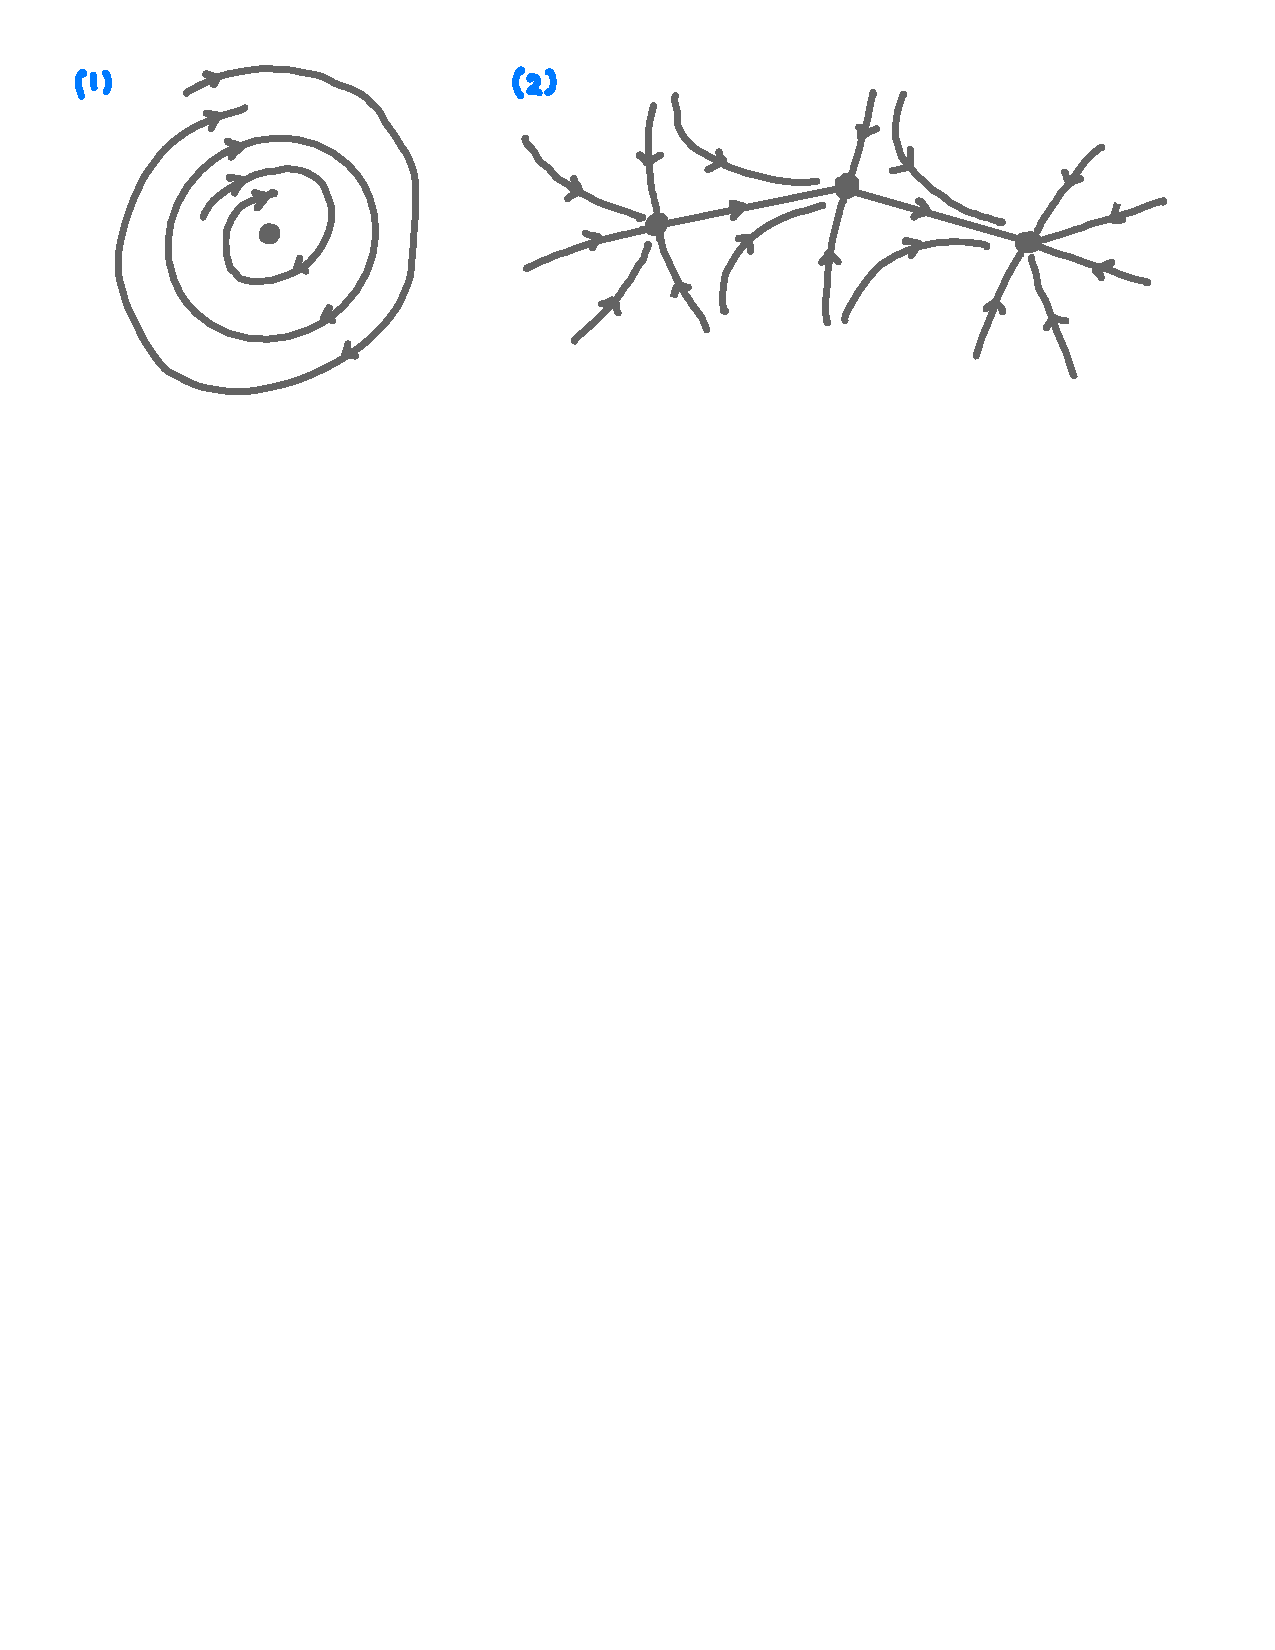
\includegraphics[width=0.9\textwidth]{Assignment_Figure_6}};

        \draw[ultra thick, red, fill, fill opacity=0.1, two marks={<}] (-5.7, -0.2) circle (1.7 and 1.6);

        \draw[ultra thick, red, marking along] (0.3, 0) -- (4, 0.7);
        \draw[ultra thick, red, marking along] (4, 0.7) -- (7, -0.3);

    \end{tikzpicture}
\end{center}

\pagebreak

%%%%%%%%%%%%%%%%%%%%%%%%%%%%%%%%

\section{The Lorenz system has an attractor}

Consider the Lorenz equations
\begin{eqnarray*}
    \dot{x} & = & \sigma (y-x) \\
    \dot{y} & = & \rho x - y - xz \\
    \dot{z} & = & - \beta z + xy
\end{eqnarray*}
for $\sigma,\beta,\rho>0$ and define the function
\[
    E(x,y,z) = x^2+y^2+(z-\rho-\sigma)^2.
\]
Show that there is a constant $R>0$ such that $E(x,y,z)$ decreases strictly along each solution $(x,y,z)(t)$ of the Lorenz equations as long as $x(t)^2+y(t)^2+z(t)^2\geq R^2$. In particular, solutions associated with any large initial condition eventually enter the ball of radius $R$, which implies that the Lorenz equations has a bounded attractor $\mathcal{A}$ inside the ball of radius $R$ for all parameter values $\sigma,\beta,\rho>0$.

\textit{Hint:} Calculate $\frac{d}{d t}(E(x(t),y(t),z(t)))$ and try to combine as many of the terms as possible using completion of the square and whichever other methods you find useful.

\color{blue}
It suffices to show that there $\exists R > 0$ such that $\frac{dE}{dt}(x, y, z) < 0$ for all $x^2 + y^2 + z^2 \geq R^2$.

\begin{align*}
    \frac{d}{dt} E(x, y, z) & = 2x \dot x + 2y \dot y  + 2(z-\rho-\sigma) \dot z                                                                                                                                                             \\
                            & = 2x \sigma (y-x) + 2y (\rho x - y - xz) + 2(z-\rho-\sigma)(-\beta z + xy)                                                                                                                                     \\
                            & = \textcolor{red}{2x \sigma y} - 2x^2 \sigma +\textcolor{red}{2y \rho x} - 2y^2 \textcolor{black}{- 2yxz} - 2\beta z^2 + \textcolor{black}{2zxy} +2\beta (\rho +\sigma)z \textcolor{red}{- 2(\rho + \sigma)xy} \\
                            & = - 2\sigma x^2 -2y^2 -2\beta z^2 + 2\beta \rho z + 2\beta\sigma z                                                                                                                                             \\
                            & = -2(\sigma x^2 + y^2) -2\beta (z^2 - (\rho+\sigma) z )                                                                                                                                                        \\
                            & = -2(\sigma x^2 + y^2) -2\beta \left(z - \frac{\rho +\sigma}{2}\right)^2 + \frac{\beta}{2}(\rho + \sigma)^2
\end{align*}

If we let $R_1 = \max\{1, \sigma, \beta\}$, then
\[-2(\sigma x^2 + y^2) -2\beta \left(z - \frac{\rho +\sigma}{2}\right)^2 + \frac{\beta}{2}(\rho + \sigma)^2 \leq -2R_1\left(x^2 + y^2 + \left(z - \frac{\rho +\sigma}{2}\right)^2\right) + \frac{\beta}{2}(\rho + \sigma)^2\]

Now choose $R_2 = \sqrt{\frac{\beta}{4R_1}(\rho + \sigma)^2}$ so
\begin{align*}
    -2R_1\left(x^2 + y^2 + \left(z - \frac{\rho +\sigma}{2}\right)^2\right) + \frac{\beta}{2}(\rho + \sigma)^2 & = -2R_1\left(x^2 + y^2 + \left(z - \frac{\rho +\sigma}{2}\right)^2\right) + 2R_1 R_2^2 \\
                                                                                                               & = -2R_1\left(x^2 + y^2 + \left(z - \frac{\rho +\sigma}{2}\right)^2 - R_2^2\right)
\end{align*}

Finally, $R_1 > 0$ so we just need
\[x^2 + y^2 + \left(z - \frac{\rho +\sigma}{2}\right)^2 - R_2^2 \geq 0 \implies x^2 + y^2 + \left(z - \frac{\rho +\sigma}{2}\right)^2 \geq R_2^2 \]
which is the equation for a sphere of radius $R_2$ centered at $(0, 0, \frac{\rho +\sigma}{2})$.

Let
\[B = \left\{(x, y, z):  x^2 + y^2 + \left(z - \frac{\rho +\sigma}{2}\right)^2 > R_2^2 \right\}\]
then from geometry,
\[B \sub \left\{(x, y, z): x^2 + y^2 + z^2 >\left(\frac{\rho +\sigma}{2} + R_2\right)^2\right\}\]

In particular, this means that if we let
\[\boxed{R > \frac{\rho + \sigma}{2}+ \sqrt{\frac{\beta}{4\max\{1, \beta, \sigma\}}(\rho + \sigma)^2}}\]
we will have $\frac{d}{dt}E < 0$ for all $x^2 + y^2 + z^2 \geq R^2$, which implies that $E$ decreases strictly on solutions of the Lorenz equations and there exists a bounded attractor $\mathcal{A}$ inside the ball of radius $R$ for all parameter values $\sigma, \beta, \rho > 0$.
\color{black}

\pagebreak

%%%%%%%%%%%%%%%%%%%%%%%%%%%%%%%%

\section{Volume of the attractor of the Lorenz system}

Consider a differential equation $\dot{u}=f(u)$ with $u=(x,y,z)\in\R^3$ and $f=(f_1,f_2,f_3)$, and denote its solutions by $u(t)=\Phi_t(u_0)$. Let $B_0$ be a ball in $\R^3$ and set $B(t):=\Phi_t(B_0)$. We denote the volume of the set $B(t)$ by $V(t)$. We have the following theorem (you do not need to prove this result): if
\[
    \mathrm{div}\, f(x,y,z) := \frac{\partial f_1}{d x}(x,y,z) + \frac{\partial f_2}{d y}(x,y,z) + \frac{\partial f_3}{d z}(x,y,z)
\]
does not depend on $(x,y,z)$, then $V(t)=V(0)\mathrm{e}^{\mathrm{div}(f)t}$.

Can you apply this result to the Lorenz equations, what is the limit of $V(t)$ as $t\to\infty$, and what does this imply for the volume of the attractor $\mathcal{A}$ of the Lorenz equations?

\color{blue}
First, we calculate the divergence of the Lorenz equations:
\begin{align*}
    \mathrm{div}\, f(x,y,z) & = \frac{\partial f_1}{d x}(x,y,z) + \frac{\partial f_2}{d y}(x,y,z) + \frac{\partial f_3}{d z}(x,y,z)                                           \\
                            & = \frac{\partial }{\partial x} (\sigma (y - x)) + \frac{\partial }{\partial y} (\rho x - y - xz) + \frac{\partial }{\partial z} (-\beta z + xy) \\
                            & = -\sigma - 1 - \beta
\end{align*}
which is indeed independent of $(x,y,z)$. Therefore, we can apply the result to the Lorenz equations.

We have
\[V(t) = V(0) e^{\text{div}(f)t} = V(0)e^{-([\sigma + \beta] t + t)}\]

Since $\sigma, \beta>0 \implies \sigma + \beta > 0$, we have that $e^{-([\sigma + \beta] t + t)}$ is positive and decreasing for all $t$.

Hence, $V(t) \to 0$. Since $V$ represents the volume of the set containing the orbit of $B_0$, we conclude that $\mathcal A$ is a point (or at least a measure zero set).
\color{black}


\end{document}